\documentclass[twoside]{book}

% Packages required by doxygen
\usepackage{calc}
\usepackage{doxygen}
\usepackage{graphicx}
\usepackage[utf8]{inputenc}
\usepackage{makeidx}
\usepackage{multicol}
\usepackage{multirow}
\usepackage{textcomp}
\usepackage[table]{xcolor}

% Font selection
\usepackage[T1]{fontenc}
\usepackage{mathptmx}
\usepackage[scaled=.90]{helvet}
\usepackage{courier}
\usepackage{amssymb}
\usepackage{sectsty}
\renewcommand{\familydefault}{\sfdefault}
\allsectionsfont{%
  \fontseries{bc}\selectfont%
  \color{darkgray}%
}
\renewcommand{\DoxyLabelFont}{%
  \fontseries{bc}\selectfont%
  \color{darkgray}%
}

% Page & text layout
\usepackage{geometry}
\geometry{%
  a4paper,%
  top=2.5cm,%
  bottom=2.5cm,%
  left=2.5cm,%
  right=2.5cm%
}
\tolerance=750
\hfuzz=15pt
\hbadness=750
\setlength{\emergencystretch}{15pt}
\setlength{\parindent}{0cm}
\setlength{\parskip}{0.2cm}
\makeatletter
\renewcommand{\paragraph}{%
  \@startsection{paragraph}{4}{0ex}{-1.0ex}{1.0ex}{%
    \normalfont\normalsize\bfseries\SS@parafont%
  }%
}
\renewcommand{\subparagraph}{%
  \@startsection{subparagraph}{5}{0ex}{-1.0ex}{1.0ex}{%
    \normalfont\normalsize\bfseries\SS@subparafont%
  }%
}
\makeatother

% Headers & footers
\usepackage{fancyhdr}
\pagestyle{fancyplain}
\fancyhead[LE]{\fancyplain{}{\bfseries\thepage}}
\fancyhead[CE]{\fancyplain{}{}}
\fancyhead[RE]{\fancyplain{}{\bfseries\leftmark}}
\fancyhead[LO]{\fancyplain{}{\bfseries\rightmark}}
\fancyhead[CO]{\fancyplain{}{}}
\fancyhead[RO]{\fancyplain{}{\bfseries\thepage}}
\fancyfoot[LE]{\fancyplain{}{}}
\fancyfoot[CE]{\fancyplain{}{}}
\fancyfoot[RE]{\fancyplain{}{\bfseries\scriptsize Generated on Thu Mar 13 2014 13:42:27 for html5sync by Doxygen }}
\fancyfoot[LO]{\fancyplain{}{\bfseries\scriptsize Generated on Thu Mar 13 2014 13:42:27 for html5sync by Doxygen }}
\fancyfoot[CO]{\fancyplain{}{}}
\fancyfoot[RO]{\fancyplain{}{}}
\renewcommand{\footrulewidth}{0.4pt}
\renewcommand{\chaptermark}[1]{%
  \markboth{#1}{}%
}
\renewcommand{\sectionmark}[1]{%
  \markright{\thesection\ #1}%
}

% Indices & bibliography
\usepackage{natbib}
\usepackage[titles]{tocloft}
\setcounter{tocdepth}{3}
\setcounter{secnumdepth}{5}
\makeindex

% Hyperlinks (required, but should be loaded last)
\usepackage{ifpdf}
\ifpdf
  \usepackage[pdftex,pagebackref=true]{hyperref}
\else
  \usepackage[ps2pdf,pagebackref=true]{hyperref}
\fi
\hypersetup{%
  colorlinks=true,%
  linkcolor=blue,%
  citecolor=blue,%
  unicode%
}

% Custom commands
\newcommand{\clearemptydoublepage}{%
  \newpage{\pagestyle{empty}\cleardoublepage}%
}


%===== C O N T E N T S =====

\begin{document}

% Titlepage & ToC
\hypersetup{pageanchor=false}
\pagenumbering{roman}
\begin{titlepage}
\vspace*{7cm}
\begin{center}%
{\Large html5sync }\\
\vspace*{1cm}
{\large Generated by Doxygen 1.8.4}\\
\vspace*{0.5cm}
{\small Thu Mar 13 2014 13:42:27}\\
\end{center}
\end{titlepage}
\clearemptydoublepage
\tableofcontents
\clearemptydoublepage
\pagenumbering{arabic}
\hypersetup{pageanchor=true}

%--- Begin generated contents ---
\chapter{Namespace Index}
\section{Namespace List}
Here is a list of all documented namespaces with brief descriptions\-:\begin{DoxyCompactList}
\item\contentsline{section}{\hyperlink{namespacecore}{core} }{\pageref{namespacecore}}{}
\item\contentsline{section}{\hyperlink{namespacehtml5sync}{html5sync} }{\pageref{namespacehtml5sync}}{}
\item\contentsline{section}{\hyperlink{namespacemodels}{models} }{\pageref{namespacemodels}}{}
\end{DoxyCompactList}

\chapter{Hierarchical Index}
\section{Class Hierarchy}
This inheritance list is sorted roughly, but not completely, alphabetically\-:\begin{DoxyCompactList}
\item \contentsline{section}{Connection}{\pageref{classConnection}}{}
\item \contentsline{section}{Dao\-Table}{\pageref{classDaoTable}}{}
\item \contentsline{section}{Database}{\pageref{classDatabase}}{}
\item \contentsline{section}{Html5\-Sync}{\pageref{classHtml5Sync}}{}
\item \contentsline{section}{Object}{\pageref{classObject}}{}
\begin{DoxyCompactList}
\item \contentsline{section}{Field}{\pageref{classField}}{}
\item \contentsline{section}{Table}{\pageref{classTable}}{}
\end{DoxyCompactList}
\item \contentsline{section}{State\-D\-B}{\pageref{classStateDB}}{}
\item \contentsline{section}{User}{\pageref{classUser}}{}
\end{DoxyCompactList}

\chapter{Class Index}
\section{Class List}
Here are the classes, structs, unions and interfaces with brief descriptions\-:\begin{DoxyCompactList}
\item\contentsline{section}{\hyperlink{classConnection}{Connection} }{\pageref{classConnection}}{}
\item\contentsline{section}{\hyperlink{classDaoTable}{Dao\-Table} }{\pageref{classDaoTable}}{}
\item\contentsline{section}{\hyperlink{classDatabase}{Database} }{\pageref{classDatabase}}{}
\item\contentsline{section}{\hyperlink{classField}{Field} }{\pageref{classField}}{}
\item\contentsline{section}{\hyperlink{classHtml5Sync}{Html5\-Sync} }{\pageref{classHtml5Sync}}{}
\item\contentsline{section}{\hyperlink{classObject}{Object} }{\pageref{classObject}}{}
\item\contentsline{section}{\hyperlink{classStateDB}{State\-D\-B} }{\pageref{classStateDB}}{}
\item\contentsline{section}{\hyperlink{classTable}{Table} }{\pageref{classTable}}{}
\item\contentsline{section}{\hyperlink{classUser}{User} }{\pageref{classUser}}{}
\end{DoxyCompactList}

\chapter{Namespace Documentation}
\hypertarget{namespacecore}{\section{core Namespace Reference}
\label{namespacecore}\index{core@{core}}
}


\subsection{Detailed Description}
\hyperlink{classConnection}{Connection} File

\hyperlink{classConnection}{Connection} Class

\begin{DoxyAuthor}{Author}
\href{https://github.com/maparrar/maqinato}{\tt https\-://github.\-com/maparrar/maqinato} 

maparrar \href{mailto:maparrar@gmail.com}{\tt maparrar@gmail.\-com}
\end{DoxyAuthor}
\hyperlink{classDatabase}{Database} File

\hyperlink{classDatabase}{Database} Class

\begin{DoxyAuthor}{Author}
\href{https://github.com/maparrar/maqinato}{\tt https\-://github.\-com/maparrar/maqinato} 

maparrar \href{mailto:maparrar@gmail.com}{\tt maparrar@gmail.\-com}
\end{DoxyAuthor}
\hyperlink{classStateDB}{State\-D\-B} File 

\hyperlink{classStateDB}{State\-D\-B} Class Clase para manejo de la base de datos de estado en S\-Q\-Lite. Esta base de datos mantiene la relación entre los usuarios y las tablas de la base de datos de la aplicación.

\begin{DoxyAuthor}{Author}
\href{https://github.com/maparrar/html5sync}{\tt https\-://github.\-com/maparrar/html5sync} 

maparrar \href{mailto:maparrar@gmail.com}{\tt maparrar@gmail.\-com}
\end{DoxyAuthor}

\hypertarget{namespacehtml5sync}{\section{html5sync Namespace Reference}
\label{namespacehtml5sync}\index{html5sync@{html5sync}}
}


\subsection{Detailed Description}
\hyperlink{classField}{Field} File  core

\hyperlink{classField}{Field} Class

\begin{DoxyAuthor}{Author}
\href{https://github.com/maparrar/html5sync}{\tt https\-://github.\-com/maparrar/html5sync} 

maparrar \href{mailto:maparrar@gmail.com}{\tt maparrar@gmail.\-com}
\end{DoxyAuthor}
core

\hyperlink{classHtml5Sync}{Html5\-Sync} File  core

\hyperlink{classHtml5Sync}{Html5\-Sync} Class

\begin{DoxyAuthor}{Author}
\href{https://github.com/maparrar/html5sync}{\tt https\-://github.\-com/maparrar/html5sync} 

maparrar \href{mailto:maparrar@gmail.com}{\tt maparrar@gmail.\-com}
\end{DoxyAuthor}
core

\hyperlink{classTable}{Table} Class Provides standard methods to Class, like J\-S\-O\-N transformations

\begin{DoxyAuthor}{Author}
\href{https://github.com/maparrar/html5sync}{\tt https\-://github.\-com/maparrar/html5sync} 

maparrar \href{mailto:maparrar@gmail.com}{\tt maparrar@gmail.\-com}
\end{DoxyAuthor}
core

\hyperlink{classTable}{Table} File  core

\hyperlink{classTable}{Table} Class

\begin{DoxyAuthor}{Author}
\href{https://github.com/maparrar/html5sync}{\tt https\-://github.\-com/maparrar/html5sync} 

maparrar \href{mailto:maparrar@gmail.com}{\tt maparrar@gmail.\-com}
\end{DoxyAuthor}
core

\hyperlink{classUser}{User} File  core

\hyperlink{classUser}{User} Class

\begin{DoxyAuthor}{Author}
\href{https://github.com/maparrar/html5sync}{\tt https\-://github.\-com/maparrar/html5sync} 

maparrar \href{mailto:maparrar@gmail.com}{\tt maparrar@gmail.\-com}
\end{DoxyAuthor}
core 
\hypertarget{namespacemodels}{\section{models Namespace Reference}
\label{namespacemodels}\index{models@{models}}
}


\subsection{Detailed Description}
\hyperlink{classObject}{Object} File  core

\hyperlink{classDaoTable}{Dao\-Table} File

\hyperlink{classDaoTable}{Dao\-Table} Class

Class data layer for the \hyperlink{classTable}{Table} class

\begin{DoxyAuthor}{Author}
\href{https://github.com/maparrar/html5sync}{\tt https\-://github.\-com/maparrar/html5sync} 

maparrar \href{mailto:maparrar@gmail.com}{\tt maparrar@gmail.\-com} 
\end{DoxyAuthor}

\chapter{Class Documentation}
\hypertarget{classConnection}{\section{Connection Class Reference}
\label{classConnection}\index{Connection@{Connection}}
}
\subsection*{Public Member Functions}
\begin{DoxyCompactItemize}
\item 
\hyperlink{classConnection_af771235bb906d236fdb9c377dd72b2d3}{\-\_\-\-\_\-construct} (\$name=\char`\"{}\char`\"{}, \$login=\char`\"{}\char`\"{}, \$password=\char`\"{}\char`\"{})
\item 
\hyperlink{classConnection_a07862558a8273ecdcb8565de4224e9d3}{set\-Name} (\$value)
\item 
\hyperlink{classConnection_a79aef948a679e22febbfcc20ab0f06cf}{set\-Login} (\$value)
\item 
\hyperlink{classConnection_a61e34cf3b6aa60c68a2f2d1a968b26e1}{set\-Password} (\$value)
\item 
\hyperlink{classConnection_a882ddaba52867a37ae4dd161a0f1126b}{get\-Name} ()
\item 
\hyperlink{classConnection_ac5ae5f832eed0233cac4e0bd822f7b5c}{get\-Login} ()
\item 
\hyperlink{classConnection_a8a2f53b314d9b93918cf83cca26c6c98}{get\-Password} ()
\end{DoxyCompactItemize}
\subsection*{Protected Attributes}
\begin{DoxyCompactItemize}
\item 
\hypertarget{classConnection_a2470d09977dda8740d324166705b98ce}{{\bfseries \$name}}\label{classConnection_a2470d09977dda8740d324166705b98ce}

\item 
\hypertarget{classConnection_ac3b5d2f7136ca52ab029e7d290b5712c}{{\bfseries \$login}}\label{classConnection_ac3b5d2f7136ca52ab029e7d290b5712c}

\item 
\hypertarget{classConnection_aab08fd521c7b1c631671094dd25b658d}{{\bfseries \$password}}\label{classConnection_aab08fd521c7b1c631671094dd25b658d}

\end{DoxyCompactItemize}


\subsection{Constructor \& Destructor Documentation}
\hypertarget{classConnection_af771235bb906d236fdb9c377dd72b2d3}{\index{Connection@{Connection}!\-\_\-\-\_\-construct@{\-\_\-\-\_\-construct}}
\index{\-\_\-\-\_\-construct@{\-\_\-\-\_\-construct}!Connection@{Connection}}
\subsubsection[{\-\_\-\-\_\-construct}]{\setlength{\rightskip}{0pt plus 5cm}Connection\-::\-\_\-\-\_\-construct (
\begin{DoxyParamCaption}
\item[{}]{\$name = {\ttfamily \char`\"{}\char`\"{}}, }
\item[{}]{\$login = {\ttfamily \char`\"{}\char`\"{}}, }
\item[{}]{\$password = {\ttfamily \char`\"{}\char`\"{}}}
\end{DoxyParamCaption}
)}}\label{classConnection_af771235bb906d236fdb9c377dd72b2d3}
Constructor 
\begin{DoxyParams}[1]{Parameters}
string & {\em \$name} & Nombre de la conexión, puede ser\-: read, write, delete, all \\
\hline
string & {\em \$login} & Login de acceso a la base de datos para la conexión \\
\hline
string & {\em \$password} & Password de acceso a la base de datos para la conexión \\
\hline
\end{DoxyParams}


\subsection{Member Function Documentation}
\hypertarget{classConnection_ac5ae5f832eed0233cac4e0bd822f7b5c}{\index{Connection@{Connection}!get\-Login@{get\-Login}}
\index{get\-Login@{get\-Login}!Connection@{Connection}}
\subsubsection[{get\-Login}]{\setlength{\rightskip}{0pt plus 5cm}Connection\-::get\-Login (
\begin{DoxyParamCaption}
{}
\end{DoxyParamCaption}
)}}\label{classConnection_ac5ae5f832eed0233cac4e0bd822f7b5c}
Getter\-: login \begin{DoxyReturn}{Returns}
string 
\end{DoxyReturn}
\hypertarget{classConnection_a882ddaba52867a37ae4dd161a0f1126b}{\index{Connection@{Connection}!get\-Name@{get\-Name}}
\index{get\-Name@{get\-Name}!Connection@{Connection}}
\subsubsection[{get\-Name}]{\setlength{\rightskip}{0pt plus 5cm}Connection\-::get\-Name (
\begin{DoxyParamCaption}
{}
\end{DoxyParamCaption}
)}}\label{classConnection_a882ddaba52867a37ae4dd161a0f1126b}
Getter\-: name \begin{DoxyReturn}{Returns}
string 
\end{DoxyReturn}
\hypertarget{classConnection_a8a2f53b314d9b93918cf83cca26c6c98}{\index{Connection@{Connection}!get\-Password@{get\-Password}}
\index{get\-Password@{get\-Password}!Connection@{Connection}}
\subsubsection[{get\-Password}]{\setlength{\rightskip}{0pt plus 5cm}Connection\-::get\-Password (
\begin{DoxyParamCaption}
{}
\end{DoxyParamCaption}
)}}\label{classConnection_a8a2f53b314d9b93918cf83cca26c6c98}
Getter\-: password \begin{DoxyReturn}{Returns}
string 
\end{DoxyReturn}
\hypertarget{classConnection_a79aef948a679e22febbfcc20ab0f06cf}{\index{Connection@{Connection}!set\-Login@{set\-Login}}
\index{set\-Login@{set\-Login}!Connection@{Connection}}
\subsubsection[{set\-Login}]{\setlength{\rightskip}{0pt plus 5cm}Connection\-::set\-Login (
\begin{DoxyParamCaption}
\item[{}]{\$value}
\end{DoxyParamCaption}
)}}\label{classConnection_a79aef948a679e22febbfcc20ab0f06cf}
Setter login 
\begin{DoxyParams}[1]{Parameters}
string & {\em \$value} & Login de acceso a la base de datos para la conexión \\
\hline
\end{DoxyParams}
\begin{DoxyReturn}{Returns}
void 
\end{DoxyReturn}
\hypertarget{classConnection_a07862558a8273ecdcb8565de4224e9d3}{\index{Connection@{Connection}!set\-Name@{set\-Name}}
\index{set\-Name@{set\-Name}!Connection@{Connection}}
\subsubsection[{set\-Name}]{\setlength{\rightskip}{0pt plus 5cm}Connection\-::set\-Name (
\begin{DoxyParamCaption}
\item[{}]{\$value}
\end{DoxyParamCaption}
)}}\label{classConnection_a07862558a8273ecdcb8565de4224e9d3}
Setter name 
\begin{DoxyParams}[1]{Parameters}
string & {\em \$value} & Nombre de la conexión, puede ser\-: read, write, delete, all \\
\hline
\end{DoxyParams}
\begin{DoxyReturn}{Returns}
void 
\end{DoxyReturn}
\hypertarget{classConnection_a61e34cf3b6aa60c68a2f2d1a968b26e1}{\index{Connection@{Connection}!set\-Password@{set\-Password}}
\index{set\-Password@{set\-Password}!Connection@{Connection}}
\subsubsection[{set\-Password}]{\setlength{\rightskip}{0pt plus 5cm}Connection\-::set\-Password (
\begin{DoxyParamCaption}
\item[{}]{\$value}
\end{DoxyParamCaption}
)}}\label{classConnection_a61e34cf3b6aa60c68a2f2d1a968b26e1}
Setter password 
\begin{DoxyParams}[1]{Parameters}
string & {\em \$value} & Password de acceso a la base de datos para la conexión \\
\hline
\end{DoxyParams}
\begin{DoxyReturn}{Returns}
void 
\end{DoxyReturn}


The documentation for this class was generated from the following file\-:\begin{DoxyCompactItemize}
\item 
server/core/Connection.\-php\end{DoxyCompactItemize}

\hypertarget{classDaoTable}{\section{Dao\-Table Class Reference}
\label{classDaoTable}\index{Dao\-Table@{Dao\-Table}}
}
\subsection*{Public Member Functions}
\begin{DoxyCompactItemize}
\item 
\hyperlink{classDaoTable_ae3a39b70effed729cbcf82ea6e7f60a8}{\-\_\-\-\_\-construct} (\$db)
\item 
\hyperlink{classDaoTable_a25515b9bb9de9478b28afb9a5737bccd}{load\-Table} (\$db\-Driver, \$table\-Name, \$mode)
\item 
\hyperlink{classDaoTable_acd70adc9314755fd650451dffb1be4de}{load\-Data} (\$table)
\item 
\hyperlink{classDaoTable_aaac575378efc5d37db3c66e3aea397b0}{check\-Data\-Changes} (\$table)
\item 
\hyperlink{classDaoTable_a8f1d51efbb72054ea54296e5756a22f4}{set\-Updated\-Column\-Mode} (\$db\-Driver, \$table)
\end{DoxyCompactItemize}
\subsection*{Protected Attributes}
\begin{DoxyCompactItemize}
\item 
\hypertarget{classDaoTable_a13c60a358bf811e03b86512e601dbeda}{{\bfseries \$db}}\label{classDaoTable_a13c60a358bf811e03b86512e601dbeda}

\item 
\hypertarget{classDaoTable_ae1e9f4416230a7e38811c1cf188ba5a2}{{\bfseries \$handler}}\label{classDaoTable_ae1e9f4416230a7e38811c1cf188ba5a2}

\end{DoxyCompactItemize}


\subsection{Constructor \& Destructor Documentation}
\hypertarget{classDaoTable_ae3a39b70effed729cbcf82ea6e7f60a8}{\index{Dao\-Table@{Dao\-Table}!\-\_\-\-\_\-construct@{\-\_\-\-\_\-construct}}
\index{\-\_\-\-\_\-construct@{\-\_\-\-\_\-construct}!DaoTable@{Dao\-Table}}
\subsubsection[{\-\_\-\-\_\-construct}]{\setlength{\rightskip}{0pt plus 5cm}Dao\-Table\-::\-\_\-\-\_\-construct (
\begin{DoxyParamCaption}
\item[{}]{\$db}
\end{DoxyParamCaption}
)}}\label{classDaoTable_ae3a39b70effed729cbcf82ea6e7f60a8}
Constructor\-: sets the database \hyperlink{classObject}{Object} and the P\-D\-O handler 
\begin{DoxyParams}[1]{Parameters}
\hyperlink{classDatabase}{Database} & {\em \$db} & database object \\
\hline
\end{DoxyParams}


\subsection{Member Function Documentation}
\hypertarget{classDaoTable_aaac575378efc5d37db3c66e3aea397b0}{\index{Dao\-Table@{Dao\-Table}!check\-Data\-Changes@{check\-Data\-Changes}}
\index{check\-Data\-Changes@{check\-Data\-Changes}!DaoTable@{Dao\-Table}}
\subsubsection[{check\-Data\-Changes}]{\setlength{\rightskip}{0pt plus 5cm}Dao\-Table\-::check\-Data\-Changes (
\begin{DoxyParamCaption}
\item[{}]{\$table}
\end{DoxyParamCaption}
)}}\label{classDaoTable_aaac575378efc5d37db3c66e3aea397b0}
Verifica si hubo cambios en una lista de tablas para un usuario 
\begin{DoxyParams}{Parameters}
{\em string\mbox{[}$\,$\mbox{]}} & \$table Nombre de la tabla que se quiere verificar \\
\hline
\end{DoxyParams}
\begin{DoxyReturn}{Returns}
boolean True si se detectaron cambios, False en otro caso 
\end{DoxyReturn}
\hypertarget{classDaoTable_acd70adc9314755fd650451dffb1be4de}{\index{Dao\-Table@{Dao\-Table}!load\-Data@{load\-Data}}
\index{load\-Data@{load\-Data}!DaoTable@{Dao\-Table}}
\subsubsection[{load\-Data}]{\setlength{\rightskip}{0pt plus 5cm}Dao\-Table\-::load\-Data (
\begin{DoxyParamCaption}
\item[{}]{\$table}
\end{DoxyParamCaption}
)}}\label{classDaoTable_acd70adc9314755fd650451dffb1be4de}
Retorna un array con los datos de la tabla (un array por registro) 
\begin{DoxyParams}[1]{Parameters}
\hyperlink{classTable}{Table} & {\em \$table} & Tabla con nombre y lista de campos \\
\hline
\end{DoxyParams}
\begin{DoxyReturn}{Returns}
array\mbox{[}\mbox{]} Array de arrays con los registros de la tabla 
\end{DoxyReturn}
\hypertarget{classDaoTable_a25515b9bb9de9478b28afb9a5737bccd}{\index{Dao\-Table@{Dao\-Table}!load\-Table@{load\-Table}}
\index{load\-Table@{load\-Table}!DaoTable@{Dao\-Table}}
\subsubsection[{load\-Table}]{\setlength{\rightskip}{0pt plus 5cm}Dao\-Table\-::load\-Table (
\begin{DoxyParamCaption}
\item[{}]{\$db\-Driver, }
\item[{}]{\$table\-Name, }
\item[{}]{\$mode}
\end{DoxyParamCaption}
)}}\label{classDaoTable_a25515b9bb9de9478b28afb9a5737bccd}
Carga una tabla de la base de datos 
\begin{DoxyParams}[1]{Parameters}
string & {\em \$db\-Driver} & Driver de la conexión a la base de datos \\
\hline
string & {\em \$table\-Name} & Nombre de la tabla que se quiere cargar \\
\hline
string & {\em \$mode} & Modo de uso de la tabla\-: ('unlock'\-: Para operaciones insert+read), ('lock'\-: Para operaciones update+delete) \\
\hline
\end{DoxyParams}
\begin{DoxyReturn}{Returns}
\hyperlink{classTable}{Table} 
\end{DoxyReturn}
\hypertarget{classDaoTable_a8f1d51efbb72054ea54296e5756a22f4}{\index{Dao\-Table@{Dao\-Table}!set\-Updated\-Column\-Mode@{set\-Updated\-Column\-Mode}}
\index{set\-Updated\-Column\-Mode@{set\-Updated\-Column\-Mode}!DaoTable@{Dao\-Table}}
\subsubsection[{set\-Updated\-Column\-Mode}]{\setlength{\rightskip}{0pt plus 5cm}Dao\-Table\-::set\-Updated\-Column\-Mode (
\begin{DoxyParamCaption}
\item[{}]{\$db\-Driver, }
\item[{}]{\$table}
\end{DoxyParamCaption}
)}}\label{classDaoTable_a8f1d51efbb72054ea54296e5756a22f4}
Define el modo Updated\-Column. Inserta una columna donde se lleva la cuenta de las insersiones y/o actualizaciones en una tabla. Crea un Trigger que realiza el proceso. 
\begin{DoxyParams}[1]{Parameters}
string & {\em \$db\-Driver} & Driver de la conexión a la base de datos \\
\hline
\hyperlink{classTable}{Table} & {\em \$table} & Tabla con nombre en la base de datos \\
\hline
\end{DoxyParams}


The documentation for this class was generated from the following file\-:\begin{DoxyCompactItemize}
\item 
server/dao/Dao\-Table.\-php\end{DoxyCompactItemize}

\hypertarget{classDatabase}{\section{Database Class Reference}
\label{classDatabase}\index{Database@{Database}}
}
\subsection*{Public Member Functions}
\begin{DoxyCompactItemize}
\item 
\hyperlink{classDatabase_a7883d28cdbffc2b417a4fbc9733fc68b}{\-\_\-\-\_\-construct} (\$name=\char`\"{}\char`\"{}, \$driver=\char`\"{}\char`\"{}, \$host=\char`\"{}\char`\"{}, \$connections=array())
\item 
\hyperlink{classDatabase_a73cb6eec277ccab50a2fa115487acbba}{set\-Name} (\$value)
\item 
\hyperlink{classDatabase_a462346c13a5fe2fb44f2b1724b538394}{set\-Driver} (\$value)
\item 
\hyperlink{classDatabase_a49df1afe26bb06f4d0cc623b95bd78ce}{set\-Host} (\$value)
\item 
\hyperlink{classDatabase_ad20b8a013d88e7204a9ead110d7a7e05}{set\-Connections} (\$value)
\item 
\hyperlink{classDatabase_ac73651dd458c78c0b8e98c5c3f47fa19}{get\-Name} ()
\item 
\hyperlink{classDatabase_a8ad30c4547ad0ed29ced3a83e6d0eff7}{get\-Driver} ()
\item 
\hyperlink{classDatabase_a66c7395bd86115c24161f96b9e7d6601}{get\-Host} ()
\item 
\hyperlink{classDatabase_aae9562910804b3fb0b14187f02ff2699}{get\-Connections} ()
\item 
\hyperlink{classDatabase_ae1081b7ad1fb0da55c3d89818cb6c48b}{add\-Connection} (\$name, \$login, \$password)
\item 
\hyperlink{classDatabase_a7c762fc601f4674513d131ea10384802}{connect} (\$connection\-Name=\char`\"{}all\char`\"{})
\end{DoxyCompactItemize}
\subsection*{Protected Attributes}
\begin{DoxyCompactItemize}
\item 
\hypertarget{classDatabase_af22161854c8f8bb14e4afa01c669fc9b}{{\bfseries \$name}}\label{classDatabase_af22161854c8f8bb14e4afa01c669fc9b}

\item 
\hypertarget{classDatabase_abaa2d02e6aafb8a9bcc711c3f5ae163f}{{\bfseries \$driver}}\label{classDatabase_abaa2d02e6aafb8a9bcc711c3f5ae163f}

\item 
\hypertarget{classDatabase_ac7fbab56b2714481177ac97d070b564f}{{\bfseries \$host}}\label{classDatabase_ac7fbab56b2714481177ac97d070b564f}

\item 
\hypertarget{classDatabase_a5b3475f4078edb1c0629ddcc00901ec7}{{\bfseries \$connections}}\label{classDatabase_a5b3475f4078edb1c0629ddcc00901ec7}

\end{DoxyCompactItemize}


\subsection{Constructor \& Destructor Documentation}
\hypertarget{classDatabase_a7883d28cdbffc2b417a4fbc9733fc68b}{\index{Database@{Database}!\-\_\-\-\_\-construct@{\-\_\-\-\_\-construct}}
\index{\-\_\-\-\_\-construct@{\-\_\-\-\_\-construct}!Database@{Database}}
\subsubsection[{\-\_\-\-\_\-construct}]{\setlength{\rightskip}{0pt plus 5cm}Database\-::\-\_\-\-\_\-construct (
\begin{DoxyParamCaption}
\item[{}]{\$name = {\ttfamily \char`\"{}\char`\"{}}, }
\item[{}]{\$driver = {\ttfamily \char`\"{}\char`\"{}}, }
\item[{}]{\$host = {\ttfamily \char`\"{}\char`\"{}}, }
\item[{}]{\$connections = {\ttfamily array()}}
\end{DoxyParamCaption}
)}}\label{classDatabase_a7883d28cdbffc2b417a4fbc9733fc68b}
Constructor 
\begin{DoxyParams}[1]{Parameters}
string & {\em \$name} & Nombre de la base de datos \\
\hline
string & {\em \$driver} & Tipo de conexión\-: mysql, oracle, postgresql \\
\hline
string & {\em \$host} & Host donde está alojada la base de datos \\
\hline
 & {\em Connection\mbox{[}$\,$\mbox{]}} & \$connections Array de conexiones a la base de datos\-: read, write, delete, all \\
\hline
\end{DoxyParams}


\subsection{Member Function Documentation}
\hypertarget{classDatabase_ae1081b7ad1fb0da55c3d89818cb6c48b}{\index{Database@{Database}!add\-Connection@{add\-Connection}}
\index{add\-Connection@{add\-Connection}!Database@{Database}}
\subsubsection[{add\-Connection}]{\setlength{\rightskip}{0pt plus 5cm}Database\-::add\-Connection (
\begin{DoxyParamCaption}
\item[{}]{\$name, }
\item[{}]{\$login, }
\item[{}]{\$password}
\end{DoxyParamCaption}
)}}\label{classDatabase_ae1081b7ad1fb0da55c3d89818cb6c48b}
Agrega una conexión a la base de datos 
\begin{DoxyParams}[1]{Parameters}
string & {\em \$name} & Nombre de la conexión\-: read, write, delete, all \\
\hline
string & {\em \$login} & Login de acceso a la base de datos para la conexión \\
\hline
string & {\em \$password} & Password de acceso a la base de datos para la conexión \\
\hline
\end{DoxyParams}
\hypertarget{classDatabase_a7c762fc601f4674513d131ea10384802}{\index{Database@{Database}!connect@{connect}}
\index{connect@{connect}!Database@{Database}}
\subsubsection[{connect}]{\setlength{\rightskip}{0pt plus 5cm}Database\-::connect (
\begin{DoxyParamCaption}
\item[{}]{\$connection\-Name = {\ttfamily \char`\"{}all\char`\"{}}}
\end{DoxyParamCaption}
)}}\label{classDatabase_a7c762fc601f4674513d131ea10384802}
Conecta con una base de datos, si hay algún error ejecuta die() para terminar cualquier proceso. 
\begin{DoxyParams}[1]{Parameters}
string & {\em \$connection\-Name} & Nombre la conexión a usar\-: read, write, delete, all \\
\hline
\end{DoxyParams}
\begin{DoxyReturn}{Returns}
P\-D\-O \hyperlink{classObject}{Object} databse handler 
\end{DoxyReturn}
\hypertarget{classDatabase_aae9562910804b3fb0b14187f02ff2699}{\index{Database@{Database}!get\-Connections@{get\-Connections}}
\index{get\-Connections@{get\-Connections}!Database@{Database}}
\subsubsection[{get\-Connections}]{\setlength{\rightskip}{0pt plus 5cm}Database\-::get\-Connections (
\begin{DoxyParamCaption}
{}
\end{DoxyParamCaption}
)}}\label{classDatabase_aae9562910804b3fb0b14187f02ff2699}
Getter\-: connections \begin{DoxyReturn}{Returns}
\hyperlink{classConnection}{Connection}\mbox{[}\mbox{]} 
\end{DoxyReturn}
\hypertarget{classDatabase_a8ad30c4547ad0ed29ced3a83e6d0eff7}{\index{Database@{Database}!get\-Driver@{get\-Driver}}
\index{get\-Driver@{get\-Driver}!Database@{Database}}
\subsubsection[{get\-Driver}]{\setlength{\rightskip}{0pt plus 5cm}Database\-::get\-Driver (
\begin{DoxyParamCaption}
{}
\end{DoxyParamCaption}
)}}\label{classDatabase_a8ad30c4547ad0ed29ced3a83e6d0eff7}
Getter\-: driver \begin{DoxyReturn}{Returns}
string 
\end{DoxyReturn}
\hypertarget{classDatabase_a66c7395bd86115c24161f96b9e7d6601}{\index{Database@{Database}!get\-Host@{get\-Host}}
\index{get\-Host@{get\-Host}!Database@{Database}}
\subsubsection[{get\-Host}]{\setlength{\rightskip}{0pt plus 5cm}Database\-::get\-Host (
\begin{DoxyParamCaption}
{}
\end{DoxyParamCaption}
)}}\label{classDatabase_a66c7395bd86115c24161f96b9e7d6601}
Getter\-: host \begin{DoxyReturn}{Returns}
string 
\end{DoxyReturn}
\hypertarget{classDatabase_ac73651dd458c78c0b8e98c5c3f47fa19}{\index{Database@{Database}!get\-Name@{get\-Name}}
\index{get\-Name@{get\-Name}!Database@{Database}}
\subsubsection[{get\-Name}]{\setlength{\rightskip}{0pt plus 5cm}Database\-::get\-Name (
\begin{DoxyParamCaption}
{}
\end{DoxyParamCaption}
)}}\label{classDatabase_ac73651dd458c78c0b8e98c5c3f47fa19}
Getter\-: name \begin{DoxyReturn}{Returns}
string 
\end{DoxyReturn}
\hypertarget{classDatabase_ad20b8a013d88e7204a9ead110d7a7e05}{\index{Database@{Database}!set\-Connections@{set\-Connections}}
\index{set\-Connections@{set\-Connections}!Database@{Database}}
\subsubsection[{set\-Connections}]{\setlength{\rightskip}{0pt plus 5cm}Database\-::set\-Connections (
\begin{DoxyParamCaption}
\item[{}]{\$value}
\end{DoxyParamCaption}
)}}\label{classDatabase_ad20b8a013d88e7204a9ead110d7a7e05}
Setter connections 
\begin{DoxyParams}{Parameters}
{\em Connection\mbox{[}$\,$\mbox{]}} & \$value Array de conexiones a la base de datos\-: read, write, delete, all \\
\hline
\end{DoxyParams}
\begin{DoxyReturn}{Returns}
void 
\end{DoxyReturn}
\hypertarget{classDatabase_a462346c13a5fe2fb44f2b1724b538394}{\index{Database@{Database}!set\-Driver@{set\-Driver}}
\index{set\-Driver@{set\-Driver}!Database@{Database}}
\subsubsection[{set\-Driver}]{\setlength{\rightskip}{0pt plus 5cm}Database\-::set\-Driver (
\begin{DoxyParamCaption}
\item[{}]{\$value}
\end{DoxyParamCaption}
)}}\label{classDatabase_a462346c13a5fe2fb44f2b1724b538394}
Setter driver 
\begin{DoxyParams}[1]{Parameters}
string & {\em \$value} & Tipo de conexión\-: mysql, oracle, postgresql \\
\hline
\end{DoxyParams}
\begin{DoxyReturn}{Returns}
void 
\end{DoxyReturn}
\hypertarget{classDatabase_a49df1afe26bb06f4d0cc623b95bd78ce}{\index{Database@{Database}!set\-Host@{set\-Host}}
\index{set\-Host@{set\-Host}!Database@{Database}}
\subsubsection[{set\-Host}]{\setlength{\rightskip}{0pt plus 5cm}Database\-::set\-Host (
\begin{DoxyParamCaption}
\item[{}]{\$value}
\end{DoxyParamCaption}
)}}\label{classDatabase_a49df1afe26bb06f4d0cc623b95bd78ce}
Setter host 
\begin{DoxyParams}[1]{Parameters}
string & {\em \$value} & Host donde está alojada la base de datos \\
\hline
\end{DoxyParams}
\begin{DoxyReturn}{Returns}
void 
\end{DoxyReturn}
\hypertarget{classDatabase_a73cb6eec277ccab50a2fa115487acbba}{\index{Database@{Database}!set\-Name@{set\-Name}}
\index{set\-Name@{set\-Name}!Database@{Database}}
\subsubsection[{set\-Name}]{\setlength{\rightskip}{0pt plus 5cm}Database\-::set\-Name (
\begin{DoxyParamCaption}
\item[{}]{\$value}
\end{DoxyParamCaption}
)}}\label{classDatabase_a73cb6eec277ccab50a2fa115487acbba}
Setter name 
\begin{DoxyParams}[1]{Parameters}
string & {\em \$value} & Nombre de la base de datos \\
\hline
\end{DoxyParams}
\begin{DoxyReturn}{Returns}
void 
\end{DoxyReturn}


The documentation for this class was generated from the following file\-:\begin{DoxyCompactItemize}
\item 
server/core/Database.\-php\end{DoxyCompactItemize}

\hypertarget{classField}{\section{Field Class Reference}
\label{classField}\index{Field@{Field}}
}
Inheritance diagram for Field\-:\begin{figure}[H]
\begin{center}
\leavevmode
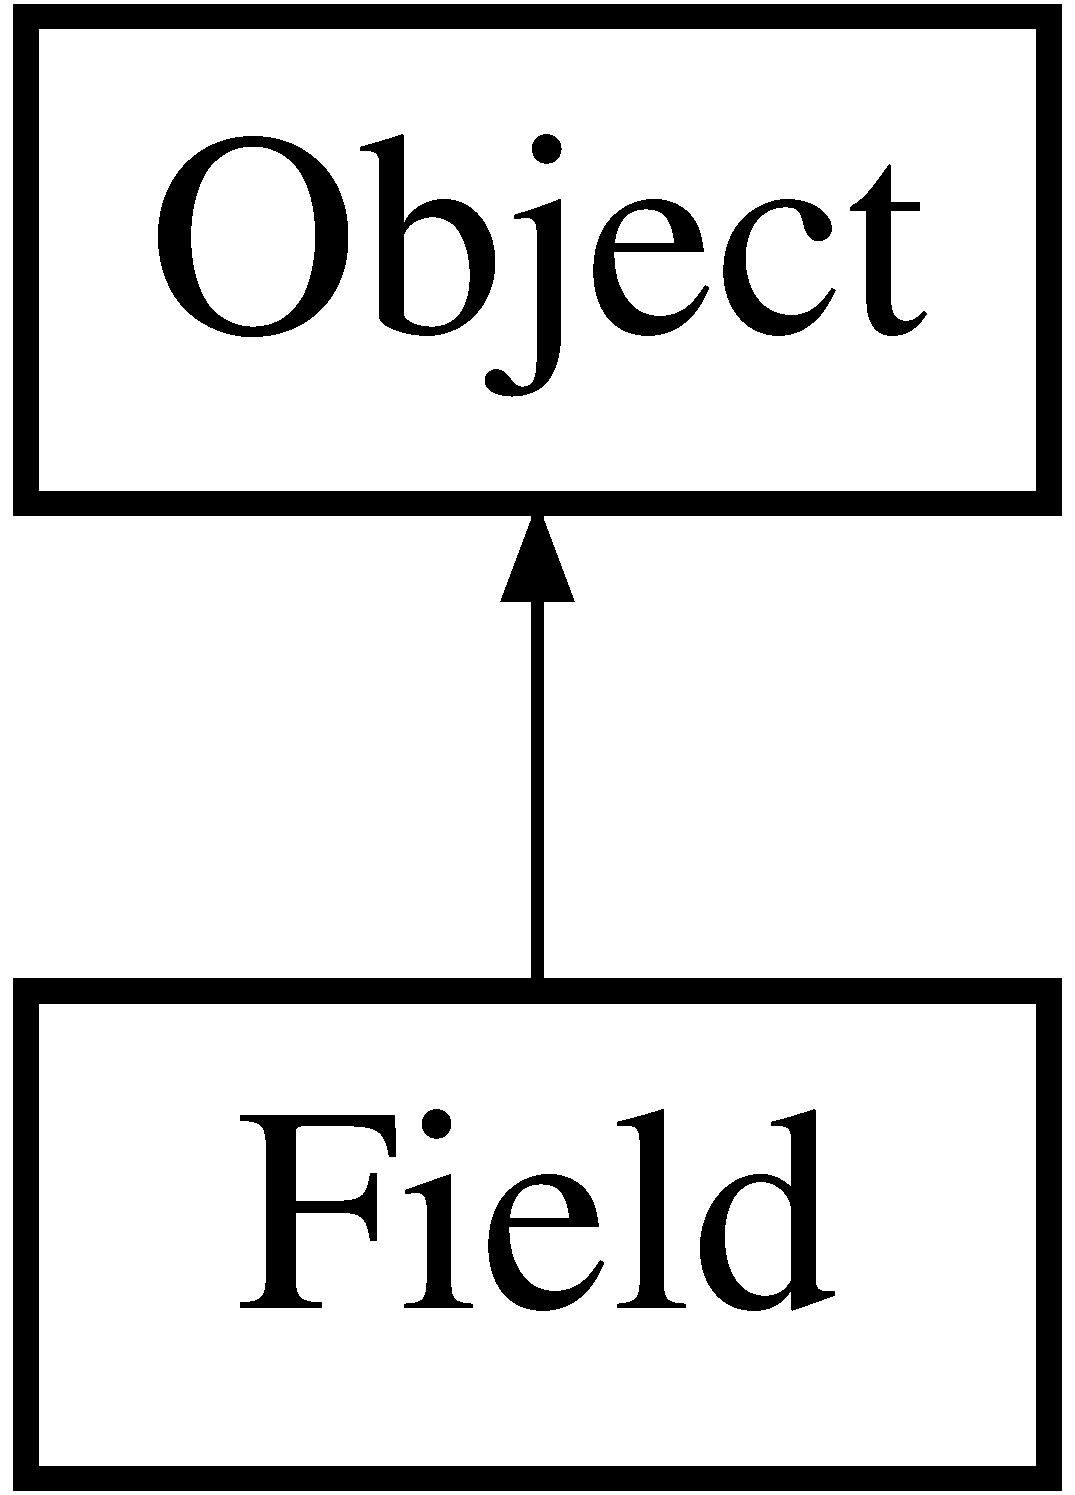
\includegraphics[height=2.000000cm]{classField}
\end{center}
\end{figure}
\subsection*{Public Member Functions}
\begin{DoxyCompactItemize}
\item 
\hyperlink{classField_af06856e25372ab1ea81a80c1594f0d44}{\-\_\-\-\_\-construct} (\$name=\char`\"{}\char`\"{}, \$type=\char`\"{}\char`\"{}, \$key=\char`\"{}\char`\"{})
\item 
\hyperlink{classField_a89957b1c6d642a6dbe15e11d3c5e3be5}{set\-Name} (\$value)
\item 
\hyperlink{classField_a724a16fc34ad198c836d90eb7de35f0d}{set\-Type} (\$value)
\item 
\hyperlink{classField_a99a515259e466f8866828b8f230261c2}{set\-Key} (\$value)
\item 
\hyperlink{classField_ac41d0cb4a99e065d98afa6a5545a5b99}{get\-Name} ()
\item 
\hyperlink{classField_af5d6650254f08096046d8818d009badb}{get\-Type} ()
\item 
\hyperlink{classField_af508c6a175be86258158d522eb0a555b}{get\-Key} ()
\end{DoxyCompactItemize}
\subsection*{Protected Attributes}
\begin{DoxyCompactItemize}
\item 
\hypertarget{classField_a27795da292b8b35025a6fccdd3c117aa}{{\bfseries \$name}}\label{classField_a27795da292b8b35025a6fccdd3c117aa}

\item 
\hypertarget{classField_a86bbb6ecadd6b39f268f68a01e21afed}{{\bfseries \$type}}\label{classField_a86bbb6ecadd6b39f268f68a01e21afed}

\item 
\hypertarget{classField_afaa0d6fab54d59423c9c892eafeae266}{{\bfseries \$key}}\label{classField_afaa0d6fab54d59423c9c892eafeae266}

\end{DoxyCompactItemize}


\subsection{Constructor \& Destructor Documentation}
\hypertarget{classField_af06856e25372ab1ea81a80c1594f0d44}{\index{Field@{Field}!\-\_\-\-\_\-construct@{\-\_\-\-\_\-construct}}
\index{\-\_\-\-\_\-construct@{\-\_\-\-\_\-construct}!Field@{Field}}
\subsubsection[{\-\_\-\-\_\-construct}]{\setlength{\rightskip}{0pt plus 5cm}Field\-::\-\_\-\-\_\-construct (
\begin{DoxyParamCaption}
\item[{}]{\$name = {\ttfamily \char`\"{}\char`\"{}}, }
\item[{}]{\$type = {\ttfamily \char`\"{}\char`\"{}}, }
\item[{}]{\$key = {\ttfamily \char`\"{}\char`\"{}}}
\end{DoxyParamCaption}
)}}\label{classField_af06856e25372ab1ea81a80c1594f0d44}
Constructor 
\begin{DoxyParams}[1]{Parameters}
string & {\em \$name} & \hyperlink{classField}{Field} Name \\
\hline
string & {\em \$type} & \hyperlink{classField}{Field} type \\
\hline
string & {\em \$key} & Kind of key of the field \\
\hline
\end{DoxyParams}


\subsection{Member Function Documentation}
\hypertarget{classField_af508c6a175be86258158d522eb0a555b}{\index{Field@{Field}!get\-Key@{get\-Key}}
\index{get\-Key@{get\-Key}!Field@{Field}}
\subsubsection[{get\-Key}]{\setlength{\rightskip}{0pt plus 5cm}Field\-::get\-Key (
\begin{DoxyParamCaption}
{}
\end{DoxyParamCaption}
)}}\label{classField_af508c6a175be86258158d522eb0a555b}
Getter\-: key \begin{DoxyReturn}{Returns}
string 
\end{DoxyReturn}
\hypertarget{classField_ac41d0cb4a99e065d98afa6a5545a5b99}{\index{Field@{Field}!get\-Name@{get\-Name}}
\index{get\-Name@{get\-Name}!Field@{Field}}
\subsubsection[{get\-Name}]{\setlength{\rightskip}{0pt plus 5cm}Field\-::get\-Name (
\begin{DoxyParamCaption}
{}
\end{DoxyParamCaption}
)}}\label{classField_ac41d0cb4a99e065d98afa6a5545a5b99}
Getter\-: name \begin{DoxyReturn}{Returns}
string 
\end{DoxyReturn}
\hypertarget{classField_af5d6650254f08096046d8818d009badb}{\index{Field@{Field}!get\-Type@{get\-Type}}
\index{get\-Type@{get\-Type}!Field@{Field}}
\subsubsection[{get\-Type}]{\setlength{\rightskip}{0pt plus 5cm}Field\-::get\-Type (
\begin{DoxyParamCaption}
{}
\end{DoxyParamCaption}
)}}\label{classField_af5d6650254f08096046d8818d009badb}
Getter\-: type \begin{DoxyReturn}{Returns}
string 
\end{DoxyReturn}
\hypertarget{classField_a99a515259e466f8866828b8f230261c2}{\index{Field@{Field}!set\-Key@{set\-Key}}
\index{set\-Key@{set\-Key}!Field@{Field}}
\subsubsection[{set\-Key}]{\setlength{\rightskip}{0pt plus 5cm}Field\-::set\-Key (
\begin{DoxyParamCaption}
\item[{}]{\$value}
\end{DoxyParamCaption}
)}}\label{classField_a99a515259e466f8866828b8f230261c2}
Setter key 
\begin{DoxyParams}[1]{Parameters}
string & {\em \$value} & Kind of key of the field \\
\hline
\end{DoxyParams}
\begin{DoxyReturn}{Returns}
void 
\end{DoxyReturn}
\hypertarget{classField_a89957b1c6d642a6dbe15e11d3c5e3be5}{\index{Field@{Field}!set\-Name@{set\-Name}}
\index{set\-Name@{set\-Name}!Field@{Field}}
\subsubsection[{set\-Name}]{\setlength{\rightskip}{0pt plus 5cm}Field\-::set\-Name (
\begin{DoxyParamCaption}
\item[{}]{\$value}
\end{DoxyParamCaption}
)}}\label{classField_a89957b1c6d642a6dbe15e11d3c5e3be5}
Setter name 
\begin{DoxyParams}[1]{Parameters}
string & {\em \$value} & \hyperlink{classField}{Field} Name \\
\hline
\end{DoxyParams}
\begin{DoxyReturn}{Returns}
void 
\end{DoxyReturn}
\hypertarget{classField_a724a16fc34ad198c836d90eb7de35f0d}{\index{Field@{Field}!set\-Type@{set\-Type}}
\index{set\-Type@{set\-Type}!Field@{Field}}
\subsubsection[{set\-Type}]{\setlength{\rightskip}{0pt plus 5cm}Field\-::set\-Type (
\begin{DoxyParamCaption}
\item[{}]{\$value}
\end{DoxyParamCaption}
)}}\label{classField_a724a16fc34ad198c836d90eb7de35f0d}
Setter type 
\begin{DoxyParams}[1]{Parameters}
string & {\em \$value} & \hyperlink{classField}{Field} type \\
\hline
\end{DoxyParams}
\begin{DoxyReturn}{Returns}
void 
\end{DoxyReturn}


The documentation for this class was generated from the following file\-:\begin{DoxyCompactItemize}
\item 
server/core/Field.\-php\end{DoxyCompactItemize}

\hypertarget{classHtml5Sync}{\section{Html5\-Sync Class Reference}
\label{classHtml5Sync}\index{Html5\-Sync@{Html5\-Sync}}
}
\subsection*{Public Member Functions}
\begin{DoxyCompactItemize}
\item 
\hyperlink{classHtml5Sync_a86e9b7a339c295ddc1c2fdfd24f13b07}{\-\_\-\-\_\-construct} (\$user)
\item 
\hyperlink{classHtml5Sync_ac2f728f1eb0459e6a8cce3ccbf17784f}{set\-Db} (\$value)
\item 
\hyperlink{classHtml5Sync_afbd2b9660431cdafc863141a6de9a7fc}{set\-User} (\$value)
\item 
\hyperlink{classHtml5Sync_aba40da5dd7d2785eb1094809339cef51}{set\-Tables} (\$value)
\item 
\hyperlink{classHtml5Sync_a97feb00b4d972988b76429f2f9e2c5b8}{set\-Parameters} (\$value)
\item 
\hyperlink{classHtml5Sync_a1356632d25bfa0b992b372fee5e3ce44}{get\-Db} ()
\item 
\hyperlink{classHtml5Sync_a9a50644c08204e15ecb09c2ab2a7d12d}{get\-User} ()
\item 
\hyperlink{classHtml5Sync_a90997b196d7a4c180e9bc4aca7323fa2}{get\-Tables} ()
\item 
\hyperlink{classHtml5Sync_ac7432fde9d8aa141f8a3436a1978cea6}{get\-Parameters} ()
\end{DoxyCompactItemize}
\subsection*{Protected Attributes}
\begin{DoxyCompactItemize}
\item 
\hypertarget{classHtml5Sync_a430e00f45a343f1efeb33b5e9af14cbb}{{\bfseries \$db}}\label{classHtml5Sync_a430e00f45a343f1efeb33b5e9af14cbb}

\item 
\hypertarget{classHtml5Sync_a8b390dbf89f49662ad72c03758f51d40}{{\bfseries \$config}}\label{classHtml5Sync_a8b390dbf89f49662ad72c03758f51d40}

\item 
\hypertarget{classHtml5Sync_aec622537a3340f5367c969c4806990cb}{{\bfseries \$user}}\label{classHtml5Sync_aec622537a3340f5367c969c4806990cb}

\item 
\hypertarget{classHtml5Sync_a438285be83079489c1d791171ad872be}{{\bfseries \$tables}}\label{classHtml5Sync_a438285be83079489c1d791171ad872be}

\item 
\hypertarget{classHtml5Sync_af93e02013382129e39e3ff472f06f6da}{{\bfseries \$parameters}}\label{classHtml5Sync_af93e02013382129e39e3ff472f06f6da}

\end{DoxyCompactItemize}


\subsection{Constructor \& Destructor Documentation}
\hypertarget{classHtml5Sync_a86e9b7a339c295ddc1c2fdfd24f13b07}{\index{Html5\-Sync@{Html5\-Sync}!\-\_\-\-\_\-construct@{\-\_\-\-\_\-construct}}
\index{\-\_\-\-\_\-construct@{\-\_\-\-\_\-construct}!Html5Sync@{Html5\-Sync}}
\subsubsection[{\-\_\-\-\_\-construct}]{\setlength{\rightskip}{0pt plus 5cm}Html5\-Sync\-::\-\_\-\-\_\-construct (
\begin{DoxyParamCaption}
\item[{}]{\$user}
\end{DoxyParamCaption}
)}}\label{classHtml5Sync_a86e9b7a339c295ddc1c2fdfd24f13b07}
Constructor 
\begin{DoxyParams}[1]{Parameters}
\hyperlink{classDatabase}{Database} & {\em \$db} & \hyperlink{classDatabase}{Database} object \\
\hline
\hyperlink{classUser}{User} & {\em \$user} & Usuario, clase manejada en \hyperlink{namespacehtml5sync}{html5sync} \\
\hline
 & {\em Table\mbox{[}$\,$\mbox{]}} & \$tables Lista de tablas del usuario \\
\hline
array & {\em \$parameters} & Parámetros de \hyperlink{namespacehtml5sync}{html5sync} \\
\hline
\end{DoxyParams}


\subsection{Member Function Documentation}
\hypertarget{classHtml5Sync_a1356632d25bfa0b992b372fee5e3ce44}{\index{Html5\-Sync@{Html5\-Sync}!get\-Db@{get\-Db}}
\index{get\-Db@{get\-Db}!Html5Sync@{Html5\-Sync}}
\subsubsection[{get\-Db}]{\setlength{\rightskip}{0pt plus 5cm}Html5\-Sync\-::get\-Db (
\begin{DoxyParamCaption}
{}
\end{DoxyParamCaption}
)}}\label{classHtml5Sync_a1356632d25bfa0b992b372fee5e3ce44}
Getter\-: db \begin{DoxyReturn}{Returns}
\hyperlink{classDatabase}{Database} 
\end{DoxyReturn}
\hypertarget{classHtml5Sync_ac7432fde9d8aa141f8a3436a1978cea6}{\index{Html5\-Sync@{Html5\-Sync}!get\-Parameters@{get\-Parameters}}
\index{get\-Parameters@{get\-Parameters}!Html5Sync@{Html5\-Sync}}
\subsubsection[{get\-Parameters}]{\setlength{\rightskip}{0pt plus 5cm}Html5\-Sync\-::get\-Parameters (
\begin{DoxyParamCaption}
{}
\end{DoxyParamCaption}
)}}\label{classHtml5Sync_ac7432fde9d8aa141f8a3436a1978cea6}
Getter\-: parameters \begin{DoxyReturn}{Returns}
array 
\end{DoxyReturn}
\hypertarget{classHtml5Sync_a90997b196d7a4c180e9bc4aca7323fa2}{\index{Html5\-Sync@{Html5\-Sync}!get\-Tables@{get\-Tables}}
\index{get\-Tables@{get\-Tables}!Html5Sync@{Html5\-Sync}}
\subsubsection[{get\-Tables}]{\setlength{\rightskip}{0pt plus 5cm}Html5\-Sync\-::get\-Tables (
\begin{DoxyParamCaption}
{}
\end{DoxyParamCaption}
)}}\label{classHtml5Sync_a90997b196d7a4c180e9bc4aca7323fa2}
Getter\-: tables \begin{DoxyReturn}{Returns}
\hyperlink{classTable}{Table}\mbox{[}\mbox{]} 
\end{DoxyReturn}
\hypertarget{classHtml5Sync_a9a50644c08204e15ecb09c2ab2a7d12d}{\index{Html5\-Sync@{Html5\-Sync}!get\-User@{get\-User}}
\index{get\-User@{get\-User}!Html5Sync@{Html5\-Sync}}
\subsubsection[{get\-User}]{\setlength{\rightskip}{0pt plus 5cm}Html5\-Sync\-::get\-User (
\begin{DoxyParamCaption}
{}
\end{DoxyParamCaption}
)}}\label{classHtml5Sync_a9a50644c08204e15ecb09c2ab2a7d12d}
Getter\-: user \begin{DoxyReturn}{Returns}
\hyperlink{classUser}{User} 
\end{DoxyReturn}
\hypertarget{classHtml5Sync_ac2f728f1eb0459e6a8cce3ccbf17784f}{\index{Html5\-Sync@{Html5\-Sync}!set\-Db@{set\-Db}}
\index{set\-Db@{set\-Db}!Html5Sync@{Html5\-Sync}}
\subsubsection[{set\-Db}]{\setlength{\rightskip}{0pt plus 5cm}Html5\-Sync\-::set\-Db (
\begin{DoxyParamCaption}
\item[{}]{\$value}
\end{DoxyParamCaption}
)}}\label{classHtml5Sync_ac2f728f1eb0459e6a8cce3ccbf17784f}
Setter db 
\begin{DoxyParams}[1]{Parameters}
\hyperlink{classDatabase}{Database} & {\em \$value} & \hyperlink{classDatabase}{Database} object \\
\hline
\end{DoxyParams}
\begin{DoxyReturn}{Returns}
void 
\end{DoxyReturn}
\hypertarget{classHtml5Sync_a97feb00b4d972988b76429f2f9e2c5b8}{\index{Html5\-Sync@{Html5\-Sync}!set\-Parameters@{set\-Parameters}}
\index{set\-Parameters@{set\-Parameters}!Html5Sync@{Html5\-Sync}}
\subsubsection[{set\-Parameters}]{\setlength{\rightskip}{0pt plus 5cm}Html5\-Sync\-::set\-Parameters (
\begin{DoxyParamCaption}
\item[{}]{\$value}
\end{DoxyParamCaption}
)}}\label{classHtml5Sync_a97feb00b4d972988b76429f2f9e2c5b8}
Setter parameters 
\begin{DoxyParams}[1]{Parameters}
array & {\em \$value} & Parámetros de \hyperlink{namespacehtml5sync}{html5sync} \\
\hline
\end{DoxyParams}
\begin{DoxyReturn}{Returns}
void 
\end{DoxyReturn}
\hypertarget{classHtml5Sync_aba40da5dd7d2785eb1094809339cef51}{\index{Html5\-Sync@{Html5\-Sync}!set\-Tables@{set\-Tables}}
\index{set\-Tables@{set\-Tables}!Html5Sync@{Html5\-Sync}}
\subsubsection[{set\-Tables}]{\setlength{\rightskip}{0pt plus 5cm}Html5\-Sync\-::set\-Tables (
\begin{DoxyParamCaption}
\item[{}]{\$value}
\end{DoxyParamCaption}
)}}\label{classHtml5Sync_aba40da5dd7d2785eb1094809339cef51}
Setter tables 
\begin{DoxyParams}{Parameters}
{\em Table\mbox{[}$\,$\mbox{]}} & \$value Lista de tablas del usuario \\
\hline
\end{DoxyParams}
\begin{DoxyReturn}{Returns}
void 
\end{DoxyReturn}
\hypertarget{classHtml5Sync_afbd2b9660431cdafc863141a6de9a7fc}{\index{Html5\-Sync@{Html5\-Sync}!set\-User@{set\-User}}
\index{set\-User@{set\-User}!Html5Sync@{Html5\-Sync}}
\subsubsection[{set\-User}]{\setlength{\rightskip}{0pt plus 5cm}Html5\-Sync\-::set\-User (
\begin{DoxyParamCaption}
\item[{}]{\$value}
\end{DoxyParamCaption}
)}}\label{classHtml5Sync_afbd2b9660431cdafc863141a6de9a7fc}
Setter user 
\begin{DoxyParams}[1]{Parameters}
\hyperlink{classUser}{User} & {\em \$value} & Usuario, clase manejada en \hyperlink{namespacehtml5sync}{html5sync} \\
\hline
\end{DoxyParams}
\begin{DoxyReturn}{Returns}
void 
\end{DoxyReturn}


The documentation for this class was generated from the following file\-:\begin{DoxyCompactItemize}
\item 
server/core/Html5\-Sync.\-php\end{DoxyCompactItemize}

\hypertarget{classObject}{\section{Object Class Reference}
\label{classObject}\index{Object@{Object}}
}
Inheritance diagram for Object\-:\begin{figure}[H]
\begin{center}
\leavevmode
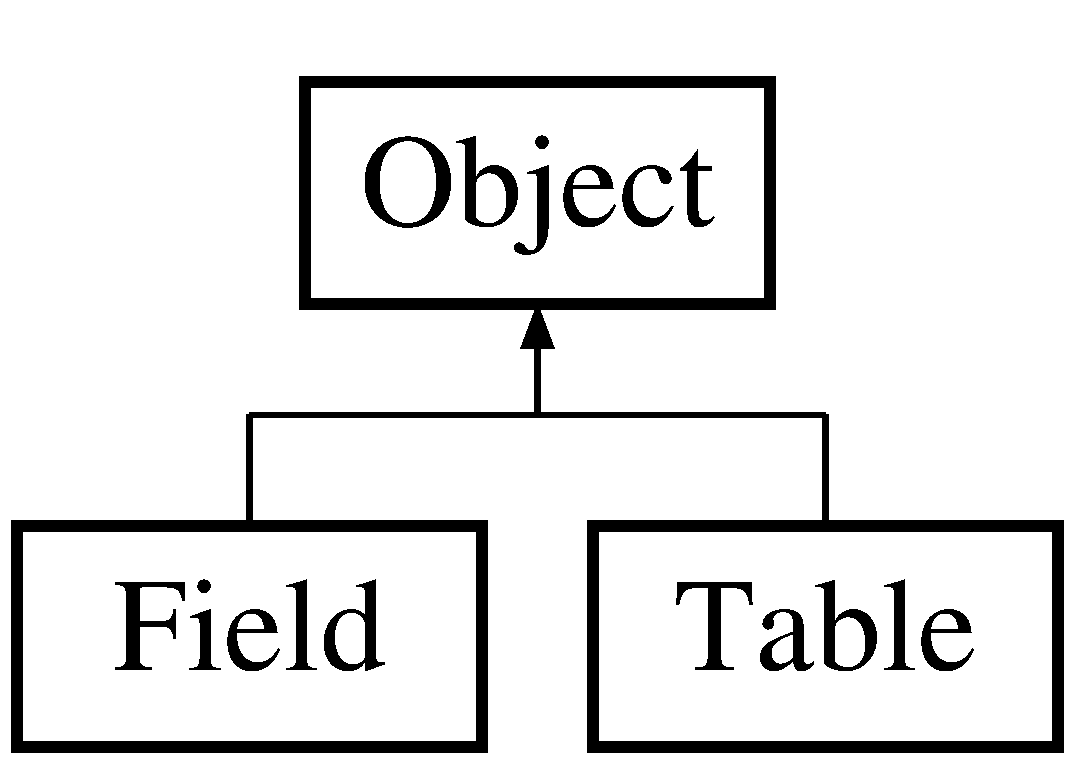
\includegraphics[height=2.000000cm]{classObject}
\end{center}
\end{figure}
\subsection*{Public Member Functions}
\begin{DoxyCompactItemize}
\item 
\hyperlink{classObject_abd44c10dee076669756ce051b952be87}{json\-Encode} ()
\end{DoxyCompactItemize}


\subsection{Member Function Documentation}
\hypertarget{classObject_abd44c10dee076669756ce051b952be87}{\index{Object@{Object}!json\-Encode@{json\-Encode}}
\index{json\-Encode@{json\-Encode}!Object@{Object}}
\subsubsection[{json\-Encode}]{\setlength{\rightskip}{0pt plus 5cm}Object\-::json\-Encode (
\begin{DoxyParamCaption}
{}
\end{DoxyParamCaption}
)}}\label{classObject_abd44c10dee076669756ce051b952be87}
Convert an object in J\-S\-O\-N format 

The documentation for this class was generated from the following file\-:\begin{DoxyCompactItemize}
\item 
server/core/Object.\-php\end{DoxyCompactItemize}

\hypertarget{classStateDB}{\section{State\-D\-B Class Reference}
\label{classStateDB}\index{State\-D\-B@{State\-D\-B}}
}
\subsection*{Public Member Functions}
\begin{DoxyCompactItemize}
\item 
\hyperlink{classStateDB_a8cafbf2a2d23683027d2133389339808}{\-\_\-\-\_\-construct} (\$path=\char`\"{}../sqlite/html5sync.\-sqlite\char`\"{})
\item 
\hyperlink{classStateDB_aabb8f09f5745735ee52f64680b6bf8cd}{set\-Path} (\$value)
\item 
\hyperlink{classStateDB_a7dfe3273772bcc8740133d8c2c7b95c5}{get\-Path} ()
\item 
\hyperlink{classStateDB_abf5cbf210df002d0802b7c22569ec2bb}{version} (\$state, \$user\-Id, \$role=\char`\"{}\char`\"{})
\end{DoxyCompactItemize}
\subsection*{Protected Attributes}
\begin{DoxyCompactItemize}
\item 
\hypertarget{classStateDB_af7ed265b88a574e5add6a2d1684839ff}{{\bfseries \$handler}}\label{classStateDB_af7ed265b88a574e5add6a2d1684839ff}

\item 
\hypertarget{classStateDB_aa6ec63a6f1117743938c32bae309fbf7}{{\bfseries \$path}}\label{classStateDB_aa6ec63a6f1117743938c32bae309fbf7}

\end{DoxyCompactItemize}


\subsection{Constructor \& Destructor Documentation}
\hypertarget{classStateDB_a8cafbf2a2d23683027d2133389339808}{\index{State\-D\-B@{State\-D\-B}!\-\_\-\-\_\-construct@{\-\_\-\-\_\-construct}}
\index{\-\_\-\-\_\-construct@{\-\_\-\-\_\-construct}!StateDB@{State\-D\-B}}
\subsubsection[{\-\_\-\-\_\-construct}]{\setlength{\rightskip}{0pt plus 5cm}State\-D\-B\-::\-\_\-\-\_\-construct (
\begin{DoxyParamCaption}
\item[{}]{\$path = {\ttfamily \char`\"{}../sqlite/html5sync.sqlite\char`\"{}}}
\end{DoxyParamCaption}
)}}\label{classStateDB_a8cafbf2a2d23683027d2133389339808}
Constructor 
\begin{DoxyParams}[1]{Parameters}
string & {\em \$path} & Ruta y nombre de la base de datos \\
\hline
\end{DoxyParams}


\subsection{Member Function Documentation}
\hypertarget{classStateDB_a7dfe3273772bcc8740133d8c2c7b95c5}{\index{State\-D\-B@{State\-D\-B}!get\-Path@{get\-Path}}
\index{get\-Path@{get\-Path}!StateDB@{State\-D\-B}}
\subsubsection[{get\-Path}]{\setlength{\rightskip}{0pt plus 5cm}State\-D\-B\-::get\-Path (
\begin{DoxyParamCaption}
{}
\end{DoxyParamCaption}
)}}\label{classStateDB_a7dfe3273772bcc8740133d8c2c7b95c5}
Getter\-: path \begin{DoxyReturn}{Returns}
string 
\end{DoxyReturn}
\hypertarget{classStateDB_aabb8f09f5745735ee52f64680b6bf8cd}{\index{State\-D\-B@{State\-D\-B}!set\-Path@{set\-Path}}
\index{set\-Path@{set\-Path}!StateDB@{State\-D\-B}}
\subsubsection[{set\-Path}]{\setlength{\rightskip}{0pt plus 5cm}State\-D\-B\-::set\-Path (
\begin{DoxyParamCaption}
\item[{}]{\$value}
\end{DoxyParamCaption}
)}}\label{classStateDB_aabb8f09f5745735ee52f64680b6bf8cd}
Setter path 
\begin{DoxyParams}[1]{Parameters}
string & {\em \$value} & Ruta y nombre de la base de datos \\
\hline
\end{DoxyParams}
\begin{DoxyReturn}{Returns}
void 
\end{DoxyReturn}
\hypertarget{classStateDB_abf5cbf210df002d0802b7c22569ec2bb}{\index{State\-D\-B@{State\-D\-B}!version@{version}}
\index{version@{version}!StateDB@{State\-D\-B}}
\subsubsection[{version}]{\setlength{\rightskip}{0pt plus 5cm}State\-D\-B\-::version (
\begin{DoxyParamCaption}
\item[{}]{\$state, }
\item[{}]{\$user\-Id, }
\item[{}]{\$role = {\ttfamily \char`\"{}\char`\"{}}}
\end{DoxyParamCaption}
)}}\label{classStateDB_abf5cbf210df002d0802b7c22569ec2bb}
Verifica para cada usuario si la estructura de las tablas ha cambiado por medio de una función de hash. Si ha cambiado, actualiza el número de versión. Si no ha cambiado, retorna el mismo número de versión. 
\begin{DoxyParams}[1]{Parameters}
string & {\em \$state} & Estructura de las tablas en J\-S\-O\-N \\
\hline
int & {\em \$user\-Id} & Id del usuario \\
\hline
string & {\em \$role} & Rol del usuario en caso de que sea nuevo \\
\hline
\end{DoxyParams}
\begin{DoxyReturn}{Returns}
int El número de la versión de la base de datos 
\end{DoxyReturn}


The documentation for this class was generated from the following file\-:\begin{DoxyCompactItemize}
\item 
server/dao/State\-D\-B.\-php\end{DoxyCompactItemize}

\hypertarget{classTable}{\section{Table Class Reference}
\label{classTable}\index{Table@{Table}}
}
Inheritance diagram for Table\-:\begin{figure}[H]
\begin{center}
\leavevmode
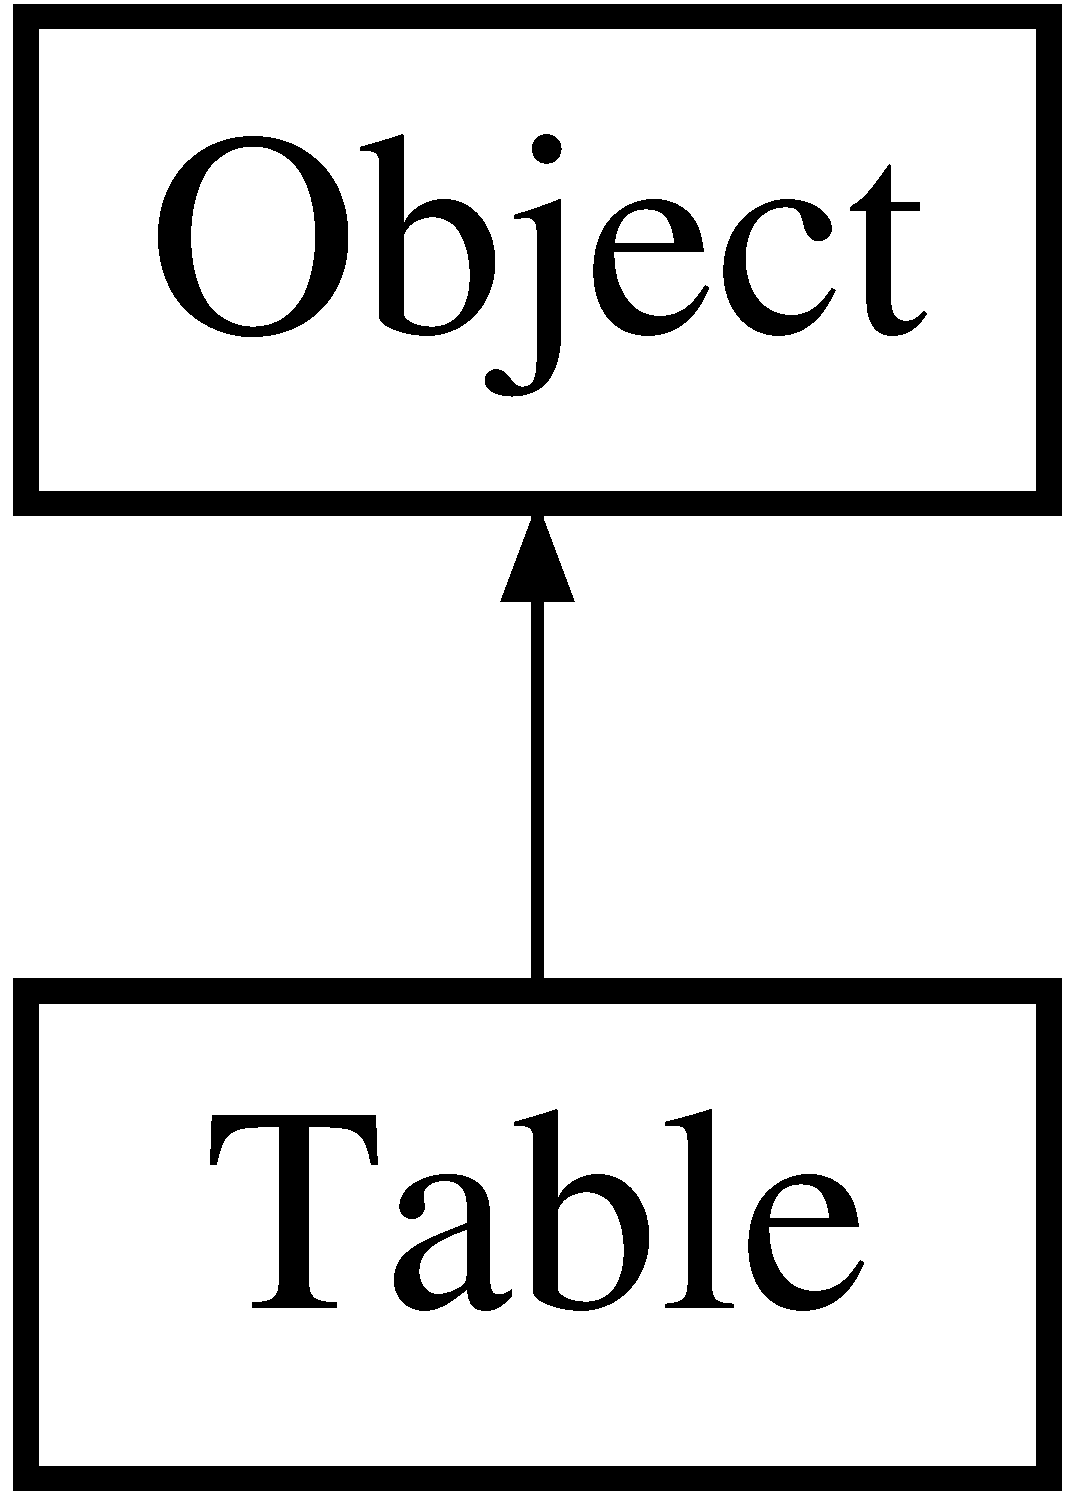
\includegraphics[height=2.000000cm]{classTable}
\end{center}
\end{figure}
\subsection*{Public Member Functions}
\begin{DoxyCompactItemize}
\item 
\hyperlink{classTable_a91623aa64ea7f31f72f467185e512aa4}{\-\_\-\-\_\-construct} (\$name=\char`\"{}\char`\"{}, \$mode=\char`\"{}\char`\"{}, \$fields=array(), \$data=array())
\item 
\hyperlink{classTable_aa0f8f35754d7d53c2583f9b06b657fa7}{set\-Name} (\$value)
\item 
\hyperlink{classTable_a26ab532f91acbfa70a0426683474beec}{set\-Mode} (\$value)
\item 
\hyperlink{classTable_afe848d39f27946d4ea1dc660efe356db}{set\-Fields} (\$value)
\item 
\hyperlink{classTable_a1ea0598b1e9ac7dff5374a9b71eff57b}{set\-Data} (\$value)
\item 
\hyperlink{classTable_a8e2ad8a066449c8fedf8f3a9192db355}{get\-Name} ()
\item 
\hyperlink{classTable_a1258d8bb455db47e49ea963f9b7f5166}{get\-Mode} ()
\item 
\hyperlink{classTable_a838132901978900cdf8c6399fd13f219}{get\-Fields} ()
\item 
\hyperlink{classTable_ad04390b230c6a2a911d0812779a7e698}{get\-Data} ()
\item 
\hyperlink{classTable_af1378aceb18290d444c34e3e75150235}{get\-Pk} ()
\end{DoxyCompactItemize}
\subsection*{Protected Attributes}
\begin{DoxyCompactItemize}
\item 
\hypertarget{classTable_a7c7f5d88257a02dd1fbeee22a77c7f39}{{\bfseries \$name}}\label{classTable_a7c7f5d88257a02dd1fbeee22a77c7f39}

\item 
\hypertarget{classTable_a03178ddf2cb8e5333712f4b3e98a1887}{{\bfseries \$mode}}\label{classTable_a03178ddf2cb8e5333712f4b3e98a1887}

\item 
\hypertarget{classTable_ab93d4088a554c8b47cb854229b83fbfb}{{\bfseries \$fields}}\label{classTable_ab93d4088a554c8b47cb854229b83fbfb}

\item 
\hypertarget{classTable_aa14f816eb8c78233ceb451fd18f69645}{{\bfseries \$data}}\label{classTable_aa14f816eb8c78233ceb451fd18f69645}

\end{DoxyCompactItemize}


\subsection{Constructor \& Destructor Documentation}
\hypertarget{classTable_a91623aa64ea7f31f72f467185e512aa4}{\index{Table@{Table}!\-\_\-\-\_\-construct@{\-\_\-\-\_\-construct}}
\index{\-\_\-\-\_\-construct@{\-\_\-\-\_\-construct}!Table@{Table}}
\subsubsection[{\-\_\-\-\_\-construct}]{\setlength{\rightskip}{0pt plus 5cm}Table\-::\-\_\-\-\_\-construct (
\begin{DoxyParamCaption}
\item[{}]{\$name = {\ttfamily \char`\"{}\char`\"{}}, }
\item[{}]{\$mode = {\ttfamily \char`\"{}\char`\"{}}, }
\item[{}]{\$fields = {\ttfamily array()}, }
\item[{}]{\$data = {\ttfamily array()}}
\end{DoxyParamCaption}
)}}\label{classTable_a91623aa64ea7f31f72f467185e512aa4}
Constructor 
\begin{DoxyParams}[1]{Parameters}
string & {\em \$name} & Nombre de la tabla \\
\hline
string & {\em \$mode} & Modo de uso de la tabla\-: ('unlock'\-: Para operaciones insert+read), ('lock'\-: Para operaciones update+delete) \\
\hline
array & {\em \$fields} & Array con los nombres de las columnas \\
\hline
array & {\em \$data} & Array con los datos de la tabla \\
\hline
\end{DoxyParams}


\subsection{Member Function Documentation}
\hypertarget{classTable_ad04390b230c6a2a911d0812779a7e698}{\index{Table@{Table}!get\-Data@{get\-Data}}
\index{get\-Data@{get\-Data}!Table@{Table}}
\subsubsection[{get\-Data}]{\setlength{\rightskip}{0pt plus 5cm}Table\-::get\-Data (
\begin{DoxyParamCaption}
{}
\end{DoxyParamCaption}
)}}\label{classTable_ad04390b230c6a2a911d0812779a7e698}
Getter\-: data \begin{DoxyReturn}{Returns}
array 
\end{DoxyReturn}
\hypertarget{classTable_a838132901978900cdf8c6399fd13f219}{\index{Table@{Table}!get\-Fields@{get\-Fields}}
\index{get\-Fields@{get\-Fields}!Table@{Table}}
\subsubsection[{get\-Fields}]{\setlength{\rightskip}{0pt plus 5cm}Table\-::get\-Fields (
\begin{DoxyParamCaption}
{}
\end{DoxyParamCaption}
)}}\label{classTable_a838132901978900cdf8c6399fd13f219}
Getter\-: fields \begin{DoxyReturn}{Returns}
\hyperlink{classField}{Field}\mbox{[}\mbox{]} 
\end{DoxyReturn}
\hypertarget{classTable_a1258d8bb455db47e49ea963f9b7f5166}{\index{Table@{Table}!get\-Mode@{get\-Mode}}
\index{get\-Mode@{get\-Mode}!Table@{Table}}
\subsubsection[{get\-Mode}]{\setlength{\rightskip}{0pt plus 5cm}Table\-::get\-Mode (
\begin{DoxyParamCaption}
{}
\end{DoxyParamCaption}
)}}\label{classTable_a1258d8bb455db47e49ea963f9b7f5166}
Getter\-: mode \begin{DoxyReturn}{Returns}
string 
\end{DoxyReturn}
\hypertarget{classTable_a8e2ad8a066449c8fedf8f3a9192db355}{\index{Table@{Table}!get\-Name@{get\-Name}}
\index{get\-Name@{get\-Name}!Table@{Table}}
\subsubsection[{get\-Name}]{\setlength{\rightskip}{0pt plus 5cm}Table\-::get\-Name (
\begin{DoxyParamCaption}
{}
\end{DoxyParamCaption}
)}}\label{classTable_a8e2ad8a066449c8fedf8f3a9192db355}
Getter\-: name \begin{DoxyReturn}{Returns}
string 
\end{DoxyReturn}
\hypertarget{classTable_af1378aceb18290d444c34e3e75150235}{\index{Table@{Table}!get\-Pk@{get\-Pk}}
\index{get\-Pk@{get\-Pk}!Table@{Table}}
\subsubsection[{get\-Pk}]{\setlength{\rightskip}{0pt plus 5cm}Table\-::get\-Pk (
\begin{DoxyParamCaption}
{}
\end{DoxyParamCaption}
)}}\label{classTable_af1378aceb18290d444c34e3e75150235}
Return the table P\-K \begin{DoxyReturn}{Returns}
\hyperlink{classField}{Field} 
\end{DoxyReturn}
\hypertarget{classTable_a1ea0598b1e9ac7dff5374a9b71eff57b}{\index{Table@{Table}!set\-Data@{set\-Data}}
\index{set\-Data@{set\-Data}!Table@{Table}}
\subsubsection[{set\-Data}]{\setlength{\rightskip}{0pt plus 5cm}Table\-::set\-Data (
\begin{DoxyParamCaption}
\item[{}]{\$value}
\end{DoxyParamCaption}
)}}\label{classTable_a1ea0598b1e9ac7dff5374a9b71eff57b}
Setter data 
\begin{DoxyParams}[1]{Parameters}
array & {\em \$value} & Array con los datos de la tabla \\
\hline
\end{DoxyParams}
\begin{DoxyReturn}{Returns}
void 
\end{DoxyReturn}
\hypertarget{classTable_afe848d39f27946d4ea1dc660efe356db}{\index{Table@{Table}!set\-Fields@{set\-Fields}}
\index{set\-Fields@{set\-Fields}!Table@{Table}}
\subsubsection[{set\-Fields}]{\setlength{\rightskip}{0pt plus 5cm}Table\-::set\-Fields (
\begin{DoxyParamCaption}
\item[{}]{\$value}
\end{DoxyParamCaption}
)}}\label{classTable_afe848d39f27946d4ea1dc660efe356db}
Setter fields 
\begin{DoxyParams}{Parameters}
{\em Field\mbox{[}$\,$\mbox{]}} & \$value \hyperlink{classField}{Field} objects of the table \\
\hline
\end{DoxyParams}
\begin{DoxyReturn}{Returns}
void 
\end{DoxyReturn}
\hypertarget{classTable_a26ab532f91acbfa70a0426683474beec}{\index{Table@{Table}!set\-Mode@{set\-Mode}}
\index{set\-Mode@{set\-Mode}!Table@{Table}}
\subsubsection[{set\-Mode}]{\setlength{\rightskip}{0pt plus 5cm}Table\-::set\-Mode (
\begin{DoxyParamCaption}
\item[{}]{\$value}
\end{DoxyParamCaption}
)}}\label{classTable_a26ab532f91acbfa70a0426683474beec}
Setter mode 
\begin{DoxyParams}[1]{Parameters}
string & {\em \$value} & Modo de uso de la tabla\-: ('unlock'\-: Para operaciones insert+read), ('lock'\-: Para operaciones update+delete) \\
\hline
\end{DoxyParams}
\begin{DoxyReturn}{Returns}
void 
\end{DoxyReturn}
\hypertarget{classTable_aa0f8f35754d7d53c2583f9b06b657fa7}{\index{Table@{Table}!set\-Name@{set\-Name}}
\index{set\-Name@{set\-Name}!Table@{Table}}
\subsubsection[{set\-Name}]{\setlength{\rightskip}{0pt plus 5cm}Table\-::set\-Name (
\begin{DoxyParamCaption}
\item[{}]{\$value}
\end{DoxyParamCaption}
)}}\label{classTable_aa0f8f35754d7d53c2583f9b06b657fa7}
Setter name 
\begin{DoxyParams}[1]{Parameters}
string & {\em \$value} & Nombre de la tabla \\
\hline
\end{DoxyParams}
\begin{DoxyReturn}{Returns}
void 
\end{DoxyReturn}


The documentation for this class was generated from the following file\-:\begin{DoxyCompactItemize}
\item 
server/core/Table.\-php\end{DoxyCompactItemize}

\hypertarget{classUser}{\section{User Class Reference}
\label{classUser}\index{User@{User}}
}
\subsection*{Public Member Functions}
\begin{DoxyCompactItemize}
\item 
\hyperlink{classUser_adb0101f8cfd611802617a78c04a6bda0}{\-\_\-\-\_\-construct} (\$id=0, \$role=\char`\"{}\char`\"{})
\item 
\hyperlink{classUser_a73a3de1fc55fc5fa1444effcb35fa0b7}{set\-Id} (\$value)
\item 
\hyperlink{classUser_ae06a7d79c33af2f6df0a4906add6c0ce}{set\-Role} (\$value)
\item 
\hyperlink{classUser_a39ad6e655fcc40623b9af2203cd7afa5}{get\-Id} ()
\item 
\hyperlink{classUser_a48631449aeb5aa95800fa8f3a17eac11}{get\-Role} ()
\end{DoxyCompactItemize}
\subsection*{Protected Attributes}
\begin{DoxyCompactItemize}
\item 
\hypertarget{classUser_a440b33833fb19a5caeb85b2e8eae3656}{{\bfseries \$id}}\label{classUser_a440b33833fb19a5caeb85b2e8eae3656}

\item 
\hypertarget{classUser_ab47cde807f0fcf85932226b162cb4520}{{\bfseries \$role}}\label{classUser_ab47cde807f0fcf85932226b162cb4520}

\end{DoxyCompactItemize}


\subsection{Constructor \& Destructor Documentation}
\hypertarget{classUser_adb0101f8cfd611802617a78c04a6bda0}{\index{User@{User}!\-\_\-\-\_\-construct@{\-\_\-\-\_\-construct}}
\index{\-\_\-\-\_\-construct@{\-\_\-\-\_\-construct}!User@{User}}
\subsubsection[{\-\_\-\-\_\-construct}]{\setlength{\rightskip}{0pt plus 5cm}User\-::\-\_\-\-\_\-construct (
\begin{DoxyParamCaption}
\item[{}]{\$id = {\ttfamily 0}, }
\item[{}]{\$role = {\ttfamily \char`\"{}\char`\"{}}}
\end{DoxyParamCaption}
)}}\label{classUser_adb0101f8cfd611802617a78c04a6bda0}
Constructor 
\begin{DoxyParams}[1]{Parameters}
int & {\em \$id} & Identificador del usuario \\
\hline
string & {\em \$role} & Rol del usuario \\
\hline
\end{DoxyParams}


\subsection{Member Function Documentation}
\hypertarget{classUser_a39ad6e655fcc40623b9af2203cd7afa5}{\index{User@{User}!get\-Id@{get\-Id}}
\index{get\-Id@{get\-Id}!User@{User}}
\subsubsection[{get\-Id}]{\setlength{\rightskip}{0pt plus 5cm}User\-::get\-Id (
\begin{DoxyParamCaption}
{}
\end{DoxyParamCaption}
)}}\label{classUser_a39ad6e655fcc40623b9af2203cd7afa5}
Getter\-: id \begin{DoxyReturn}{Returns}
int 
\end{DoxyReturn}
\hypertarget{classUser_a48631449aeb5aa95800fa8f3a17eac11}{\index{User@{User}!get\-Role@{get\-Role}}
\index{get\-Role@{get\-Role}!User@{User}}
\subsubsection[{get\-Role}]{\setlength{\rightskip}{0pt plus 5cm}User\-::get\-Role (
\begin{DoxyParamCaption}
{}
\end{DoxyParamCaption}
)}}\label{classUser_a48631449aeb5aa95800fa8f3a17eac11}
Getter\-: role \begin{DoxyReturn}{Returns}
string 
\end{DoxyReturn}
\hypertarget{classUser_a73a3de1fc55fc5fa1444effcb35fa0b7}{\index{User@{User}!set\-Id@{set\-Id}}
\index{set\-Id@{set\-Id}!User@{User}}
\subsubsection[{set\-Id}]{\setlength{\rightskip}{0pt plus 5cm}User\-::set\-Id (
\begin{DoxyParamCaption}
\item[{}]{\$value}
\end{DoxyParamCaption}
)}}\label{classUser_a73a3de1fc55fc5fa1444effcb35fa0b7}
Setter id 
\begin{DoxyParams}[1]{Parameters}
int & {\em \$value} & Identificador del usuario \\
\hline
\end{DoxyParams}
\begin{DoxyReturn}{Returns}
void 
\end{DoxyReturn}
\hypertarget{classUser_ae06a7d79c33af2f6df0a4906add6c0ce}{\index{User@{User}!set\-Role@{set\-Role}}
\index{set\-Role@{set\-Role}!User@{User}}
\subsubsection[{set\-Role}]{\setlength{\rightskip}{0pt plus 5cm}User\-::set\-Role (
\begin{DoxyParamCaption}
\item[{}]{\$value}
\end{DoxyParamCaption}
)}}\label{classUser_ae06a7d79c33af2f6df0a4906add6c0ce}
Setter role 
\begin{DoxyParams}[1]{Parameters}
string & {\em \$value} & Rol del usuario \\
\hline
\end{DoxyParams}
\begin{DoxyReturn}{Returns}
void 
\end{DoxyReturn}


The documentation for this class was generated from the following file\-:\begin{DoxyCompactItemize}
\item 
server/core/User.\-php\end{DoxyCompactItemize}

%--- End generated contents ---

% Index
\newpage
\phantomsection
\addcontentsline{toc}{part}{Index}
\printindex

\end{document}
